 \section{Разработка принципиальной схемы усилителя мощности}

 \textbf{\subsection{Разработка и расчёт принципиальной схемы
 усилителя мощности}}
  \vspace{1em}
  \begin{figure}[htbp]
    \center{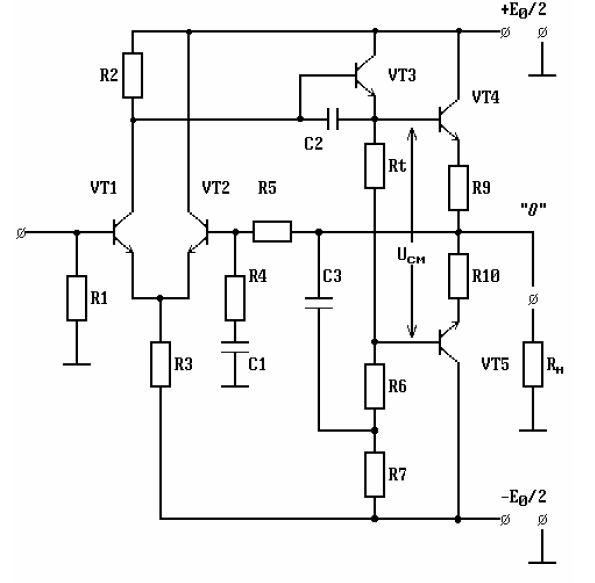
\includegraphics[width=0.8\linewidth]{picture_3}}
    \caption{Электрическая принципиальная схема усилителя}
    \label{figure:p2_1}
  \end{figure}

 \textbf{\subsection{Выбор цепи термостабилизации}}
  \vspace{1em}
  Цепь предназначена  для  создания  начального  смещения  на базах транзисторов выходного каскада. В процессе нагрева их параметры существенно изменяются, что влечет за собой изменение режимов и нарушение работы  всей  схемы. Цепь термостабилизации  в  зависимости  от  температурного  режима  изменяет  напряжение  смещения  так,  чтобы  компенсировать  изменение  параметров  транзисторов.\par

  Используем схему цепи термостабилизации, представленную на рисунке 2.2.\par
  Диапазон рабочих температур $-20\ldots +50~^0C$. 
